
% new page to start the paper
\newpage

\section{Introduction}
In Brain-Computer Interfaces (BCIs), discerning the relevance of a given signal interval is incredibly challenging.
Countless studies focus on that discernment process, but knowledge of the context a signal was recorded in is often unavailable.
Details like the specific recording device used, the sampling rate, electrode placement, and biometric information about the subject can all influence the signal and yet are all frequently lost information in many published works.\cite{Review}
It is then easy to reason that reconstructing this contextual information has the potential to greatly improve many research works, as this opens up the possibility of easily identifying patterns in the data that are hidden without this thorough labeling.
But mapping out how to perform this information reconstruction is a tough challenge, with obvious hurdles like the lack of labeled data to consider in the first place.

In this paper, we will review a recent study by Arnau-Gonzalez et al. \cite{ES1D} that uses a deep neural network to identify specific subjects from a given set based on their EEG data.
ES1D utilized a publicly available dataset from a publication called ``DREAMER: A Database for Emotion Recognition Through EEG and ECG Signals From Wireless Low-cost Off-the-Shelf Devices
'' \cite{DREAMER}. The model proposed in the ES1D paper was able to consistently outperform traditional classifiers, with subject identification accuracy of about 94\%\cite{ES1D}.
Background works related to the topic of subject identification along with other works related to ES1D are discussed in this paper to give context as to why the model worked so well.
We then review an attempt at recreating the proposed ES1D model and compare its performance on a similar dataset with a narrower classification focus.
The results of this recreation were far lower than those reported in the original ES1D paper, so we will go in depth as to why what may be.

\section{Background and Related Work}
Before reviewing the related works, it is important that the list of contextual information is layed out clearly.
Notably that the EEG dataset used in ES1D (DREAMER\cite{DREAMER}) was collected using a low-quality device and aimed to record Event-Related Potential (ERP) data for emotion recognition.
Neither emotion recognition, nor ERP recordings are the focus of the ES1D model. But these are important to mention because ERPs have been shown to correlate well with biometric information, such as age and gender, both of which DREAMER had labeled.
This correlation could potentially influence the accuracy of ES1D's results, so it is important to mention.
As we explore the impact of contextual influences and methodology while reviewing the related works, consider the factors mentioned here.
\subsection{CEREBRE}
The CEREBRE paper\cite{Cerebre} laid the foundation for many other works we will discuss in this paper.
The reason so many works found it to be so influential was becasue of its focus on the classification link between ERP and biometric information, or as they called it ``Cognitive Event-RElated
Biometric REcognition'', or CEREBRE for short. But their focus was entirely on the ERP, not an entire EEG signal.
This study was engineered with immense consideration of the influence that experimental modalities can play, and as such, their classification accuracy was high without claims that it will generalize well.
The devices used to collect EEG signals in this study were also high quality, with a sampling rate of 500 Hz and a total of 32 electrode channels.
ES1D can be seen as a natural extension of CEREBRE, with an emphasis on generalization. Instead of just focusing on the ERPs, ES1D wants to consider the whole signal.
Rather than engineering the study strongly to suit the given experimental parameters, ES1D tries to create a model that will fit any case.
And while CEREBRE aims to eliminate noise from the recording process by using top tier equipment, ES1D embraces the noise and aims to classify despite its presence.
\subsection{DREAMER Dataset}
The DREAMER dataset\cite{DREAMER} was used in ES1D to train and test the model. 
Its focus was on recording ERPs for emotion recognition, but the data had included more specific labels than most works normally would.
See figure \ref{fig:dreamer} for a list of the labels included in the dataset. 
As mentioned before, the data was collected on a low-quality device, which the authors of ES1D claim adds to the credibility of their classification model results.
\begin{center}
    \begin{figure}[h]
        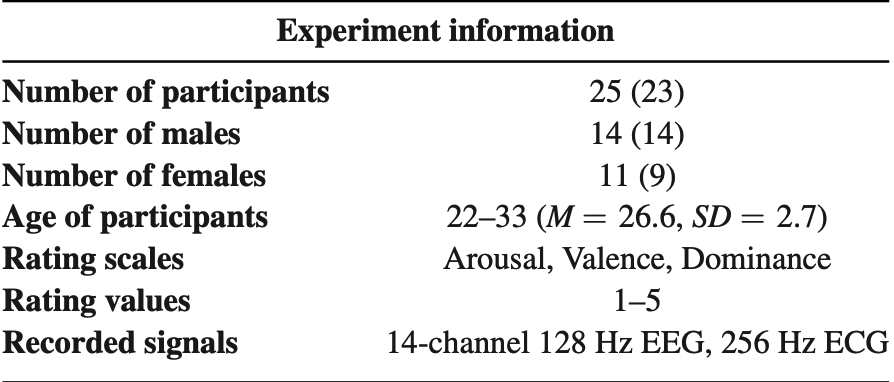
\includegraphics[width=0.5\textwidth]{dreamer_labels.png}
        \caption{\small{Labels included in DREAMER}}
        \label{fig:dreamer}
    \end{figure}
\end{center}
\subsection{Brainprint}
The Brainprint study\cite{Brainprint} is nearly identical to ES1D in its focus, but the methodology they utilized differs slightly.
ES1D has sets of recordings from 23 subjects, all recorded in a single session. Brainprint, on the other hand, took recordings from subjects over many months.
The lag and fluctuation of ERPs and the impact this can have on their classification accuracy is reviewed in the Brainprint paper, but the authors show that this can be accomodated and accounted for.
Their study only focused on three EEG channels, as opposed to the 14 channels used in ES1D.
Where Brainprint stops short of ES1D is in their development of a new classification model.
Their study does not introduce a new model, but instead uses a suite of traditional models (Cross-correlation, Divergent Autoencoder, Naive Discriminant Learning, and Support Vector Machine) to classify the data.

\subsection{Transformer Networks}
This paper, ``Efficacy of Transformer Networks for Classification of Raw EEG Data''\cite{TransformerNetworks} is a recent study that utilized Transformers to classify EEG data.
While the methodology is entirely different from ES1D's approach, including the nature of feature extraction in their study, it is still worth mentioning here because they separated the classification of specific biometric markers.
Their classifier was tested on its ability to predict the following from EEG data: age, gender, age and gender combined, and specific task identification.
The most important takeaway here is that the combination of age and gender was the easiest to classify, which may contribute to the success of ES1D's model since their total subject identification focus extends the number of considered features greatly.
Another interesting part about this study is that they tested their methods on different datasets and found that their accuracy held.
It should be noted that a cross comparison of datasets does not exist in the ES1D model.
\subsection{Inception Modules}
Switching focus to a study that has less to do with ES1D's focus and more to do with its model architecture, we will now review the paper ``Going Deeper with Convolutions''\cite{Inception}, published by some researchers at Google in 2014.
This paper introduced the Inception module, which is a convolutional neural network architecture that concatenates the outputs of multiple convolutional layers with different filter and kernel sizes.
This allows for the network to filter out zero values from the input weights and expand the relevant weights by directing them to their respectively sized convolutional layers.
This module setup is used in ES1D's architecture.
\section{Methods and Experimental Setup}
The recreation work attempted to follow the ES1D model as closesly as possible.
There were, however, some key components not listed in the original paper.
Additionally, some methods, like artefact removal, were performed with standard software toolkits that have since been modified.
In response to this, we aimed to recreate the model as closely as possible and write scripts to perform any missing steps.
This section will go over the entire model design and experimentation process, but a high-level overview of the preprocessing and model architecture can be found in figures \ref{fig:preprocessing} \& \ref{fig:model_architecture}.
% Figures should not  be bound by 2 column format

\begin{center}
    \begin{figure}[h]
        \centering
        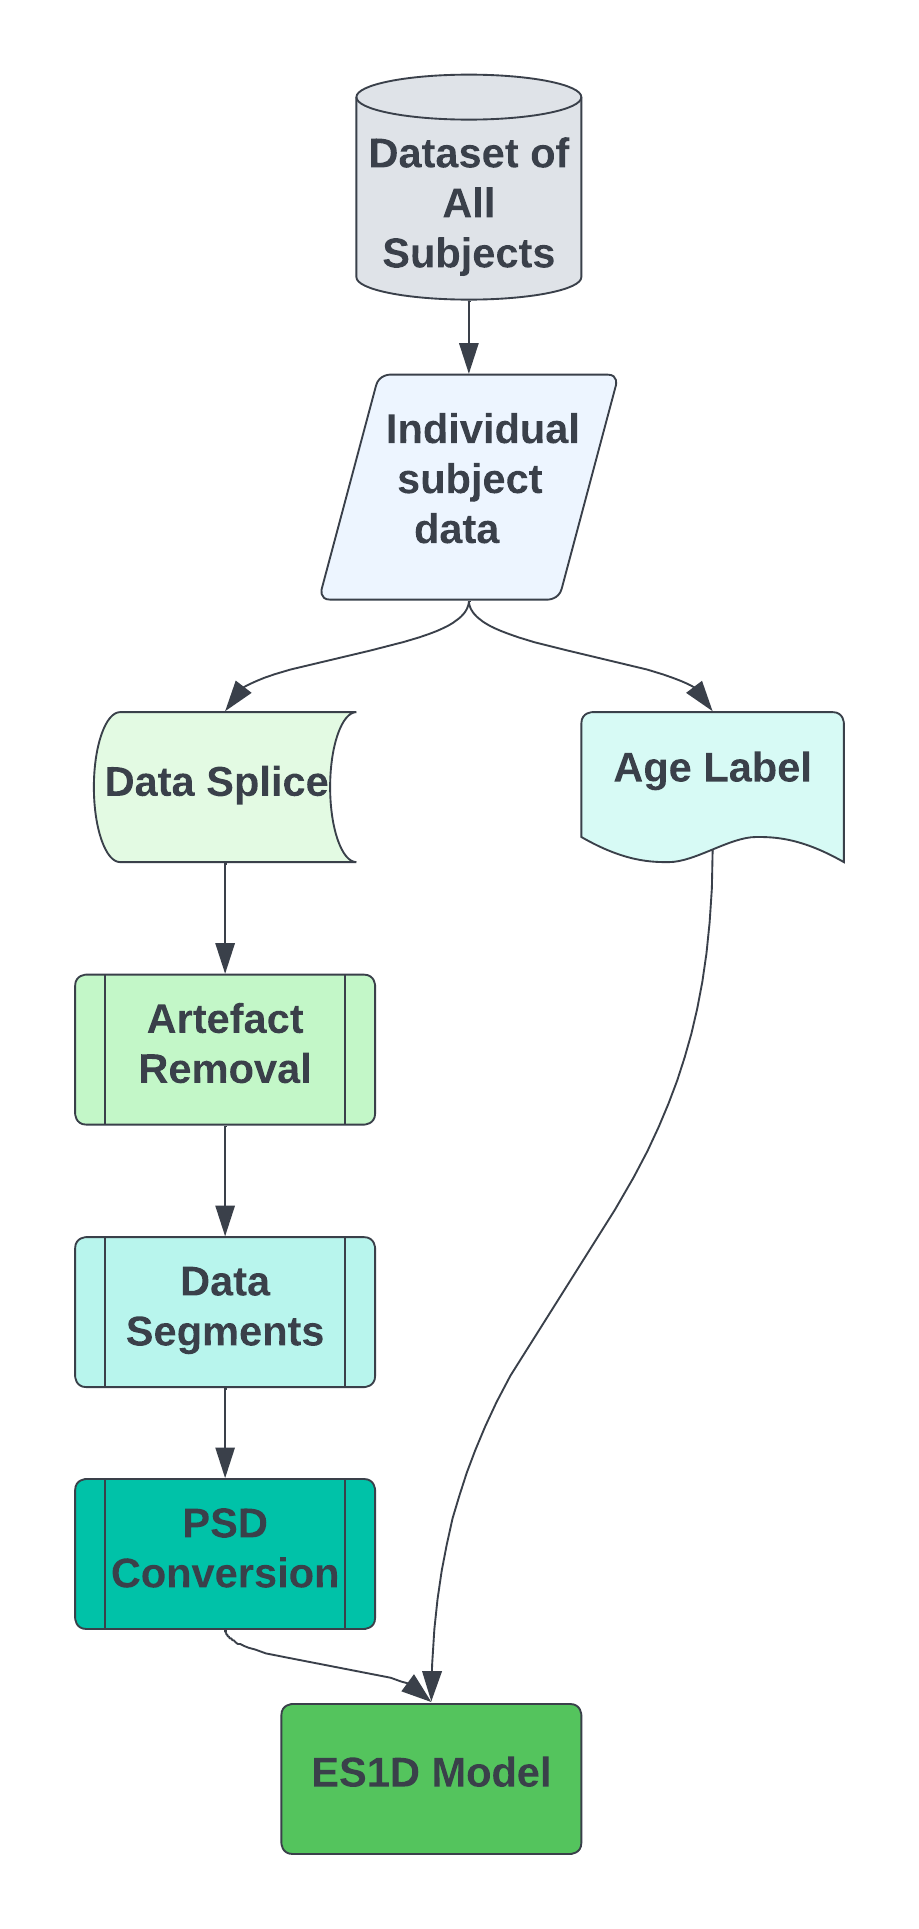
\includegraphics[width=0.3\textwidth]{data_pipeline.png}
        \caption{\small{Preprocessing Pipeline}}
        \label{fig:preprocessing}
    \end{figure}
    \begin{figure}[h]
        \centering

        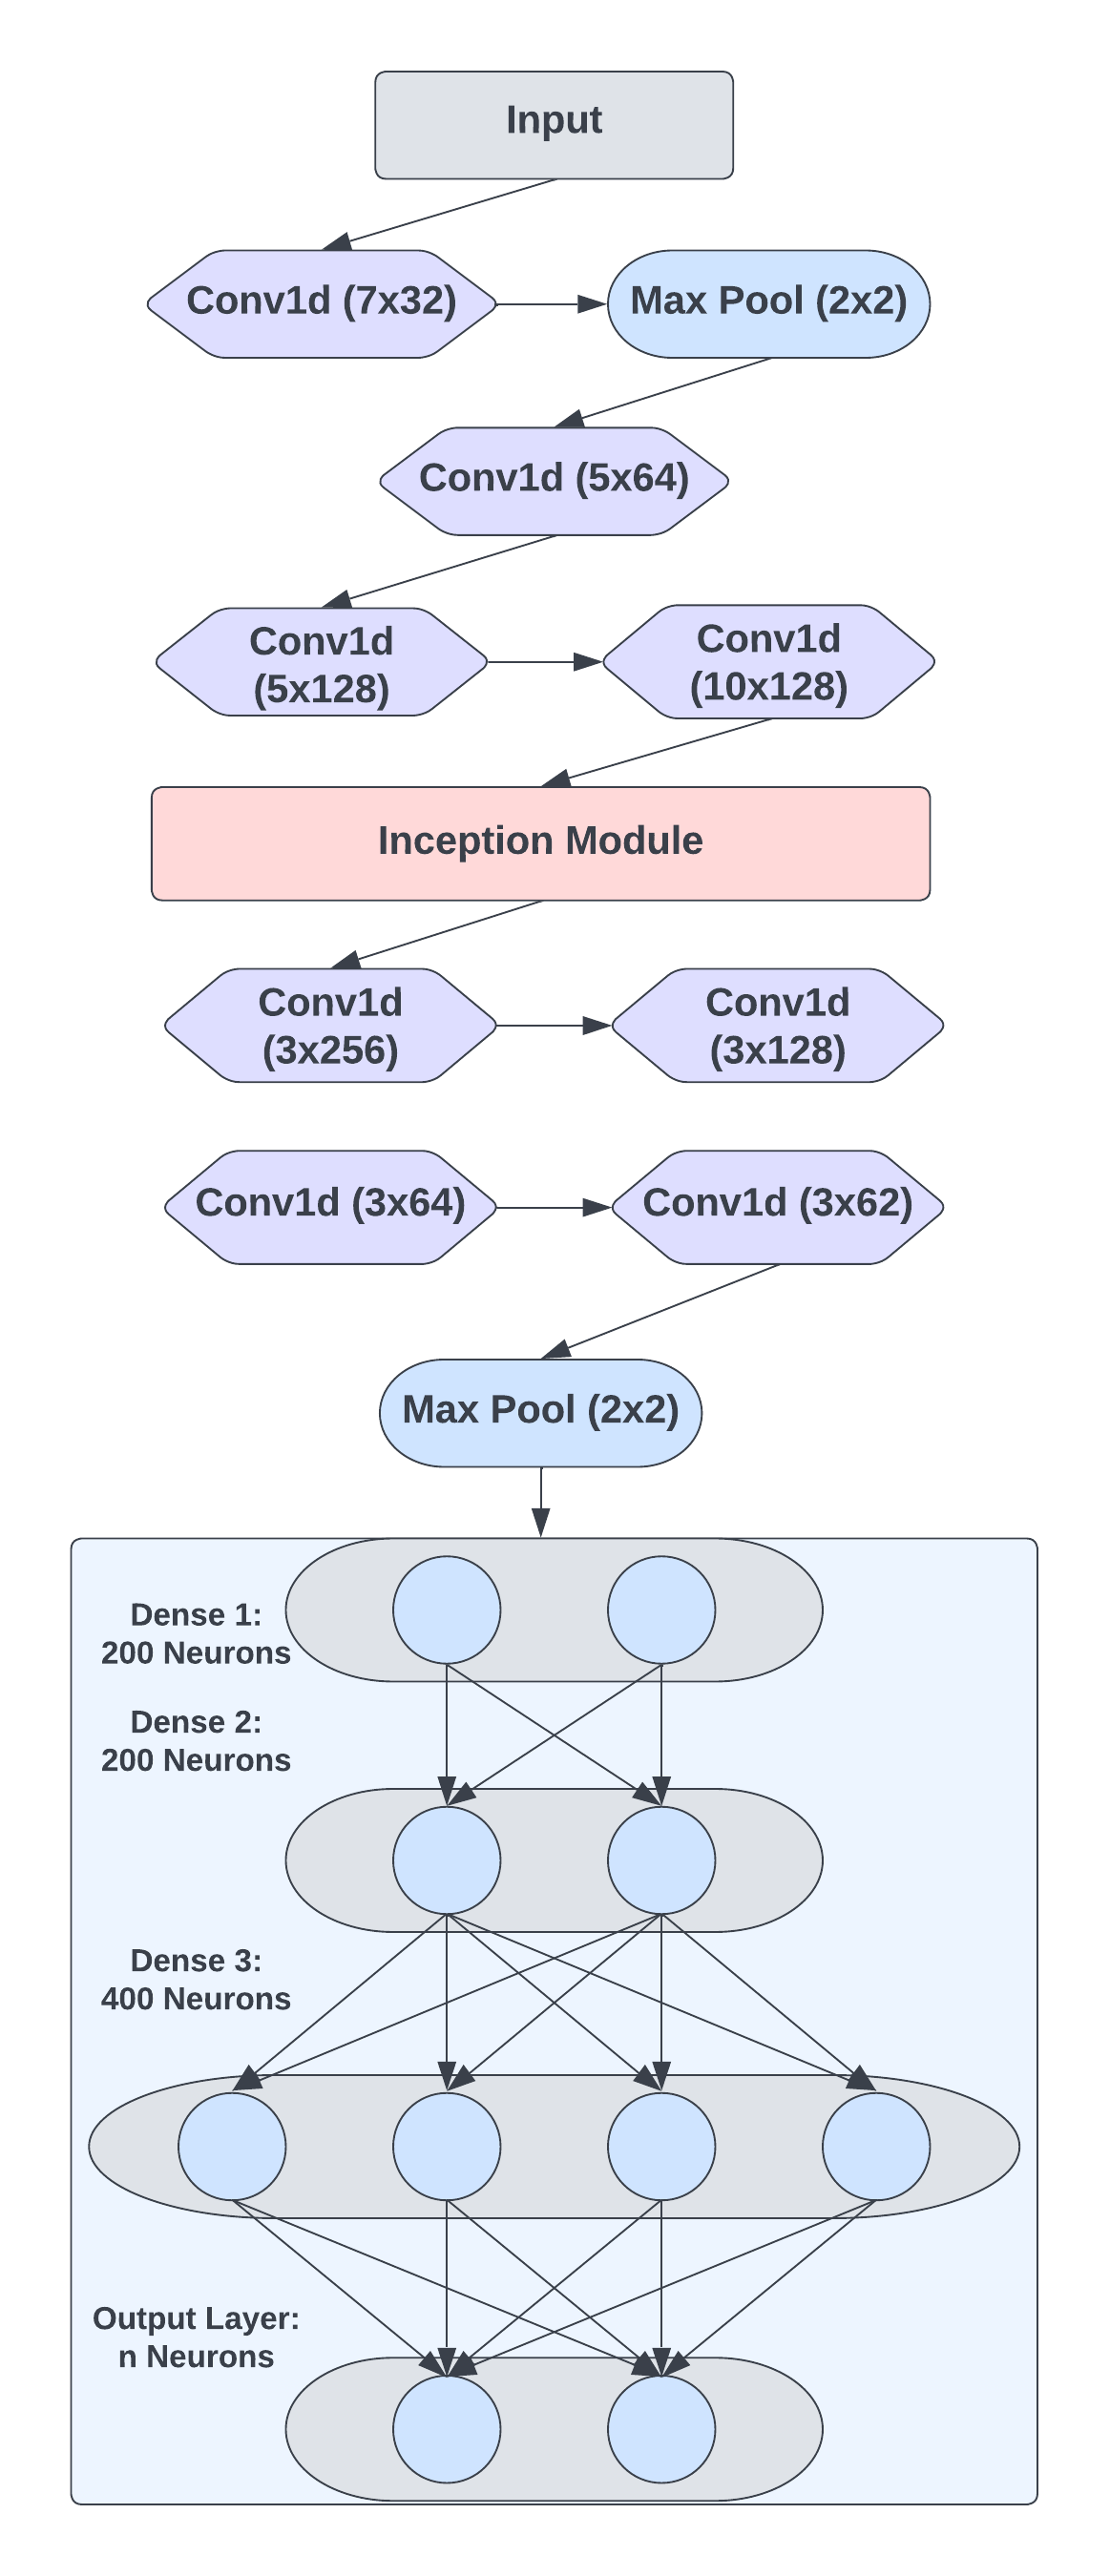
\includegraphics[width=0.3\textwidth]{ES1D.png}
        \caption{\small{Model Architecture}}
        \label{fig:model_architecture}
    \end{figure}
\end{center}

\subsection{Dataset}
The dataset used in the recreation was not the same one used in the ES1D paper. Instead, \href{https://www.kaggle.com/datasets/ayurgo/data-eeg-age-v1}{a publicly available dataset} was used.
An attempt was made to replicate ES1D with the original DREAMER dataset.
The authors of ES1D did grant permission to utilize it and gave an access link for it, but the full source was nested into a single MATLAB file with no clear direction on how to handle it.
Consequently, the decision to use a public dataset that fit the same label criteria was made.

\subsection{Data Preprocessing}

The preprocessing and feature extraction steps are among the most crucial in the ES1D model and this recreation.
First, data is taken from each subject file in set sizes as predefined by the authors. For ES1D this represented 6 seconds of EEG data, which was recorded at 128 Hz.
For the recreation, the data was taken to represent 3 seconds of EEG data, which was recorded at 250 Hz.
But in both studies, a full pass on the training and evaluation data was made to grab the number of samples needed for each subject.
For each item in these sets, the age value (shown at the top of the file) was removed and stored as a separate dataframe that was kept as the second value in a tuple of the form (dataframe, age).
These training and evaluation sets were saved separately and made easily accessible using Pickle.
After the initial loading, the data needed to be filtered, but the ES1D model cited an artefact removal method that was no longer publicly available.
To handle this in the recreation, a simple bandpass filter was used on the data to remove noise. No ICA was performed as there were no instructions from the ES1D model on whether this was the correct method.
After this, the PSD was calculated for each sample and the data was normalized. The PSD was calculated using the Welch method, the formula for which is shown below.
\begin{equation}
    \label{eq:psd}
    P_{xx}(f) = \frac{1}{N} \sum_{n=0}^{N-1} |X(f_n)|^2
\end{equation}
The PSD was calculated using a window size of 256 and a stride of 128, allowing for 50\% overlap between windows.
The data was then normalized using the following formula.
\begin{equation}
    \label{eq:normalize}
    x_{norm} = \frac{x - \mu}{\sigma}
\end{equation}
The data was then split into 3 second segments, and the mean of each segment was calculated.
The mean was then subtracted from each segment, and the result was stored as a new dataframe.
This was done for each subject and the resulting dataframes were stored in a list.
The list was then converted to a numpy array and saved as a pickle file.

\subsection{Model Architecture, Parameters, and Hyperparameters}
The model architecture used in the recreation was the same as the one used in the ES1D paper.
Layer by layer details are shown in fig \ref{fig:model_architecture}, but let's discuss the more important parts of the model and what was missing from the initial paper.
The most notable distinction to begin making is that the flow of weights across the inception module is not provided in the ES1D paper.
Instead, methods had to be devised to determine the flow of weights, and ultimately, they were simply treated as concatenated layers but stored separately.
Additionally, padding and stride values were not provided in the ES1D paper, so they were set to the default values of 1 and 0 respectively.
The learning rate for the Adam optimizer was also not made clear in the paper, so in the recreation it was set to 0.001.
In the original ES1D paper, their model was trained for 1,000,000 iterations, but in the recreation, the model was trained for only 150.
Many of these hyperparameter and control values have the potential to contribute to the recreation's lack of success.

\subsection{My Contributions}
Many of my contributions were made to compensate for the missing parts listed above. 
I wrote code for filtering and feature extraction beyond the standards mentioned in the paper.
While this wasn't necessary for the experiment I generated fast fourier transform and Welch's method PSD calculation scripts from scratch, but most experiments used the standard library forms of these methods.
My recreation of the ES1D was done in Pytorch, which differed from the initial ES1D model created in Tensorflow.
It should be noted, however, that no code was supplied for the ES1D model, so the importance of the Pytorch recreation comes less from the act of writing code and more from the fact that the Inception module implementation needed to be done in a different framework, one that was not authored by the same people who created the module.
My last contribution to mention is the fact that I selected a different dataset to use for the recreation. This required a series of extra steps and scripts written for the preprocessing of the data.

\section{Results}
The recreation was not able to achieve the same classification results as the original ES1D paper, as shown by figure \ref{fig:results}.
The original ES1D paper reported an accuracy of 94\% on the DREAMER dataset, but the recreation was only able to achieve an accuracy just under 25\%.
This could be due to a number of factors, so let's review them and explain why they may have impacted our findings.

\begin{center}
    \begin{figure}
        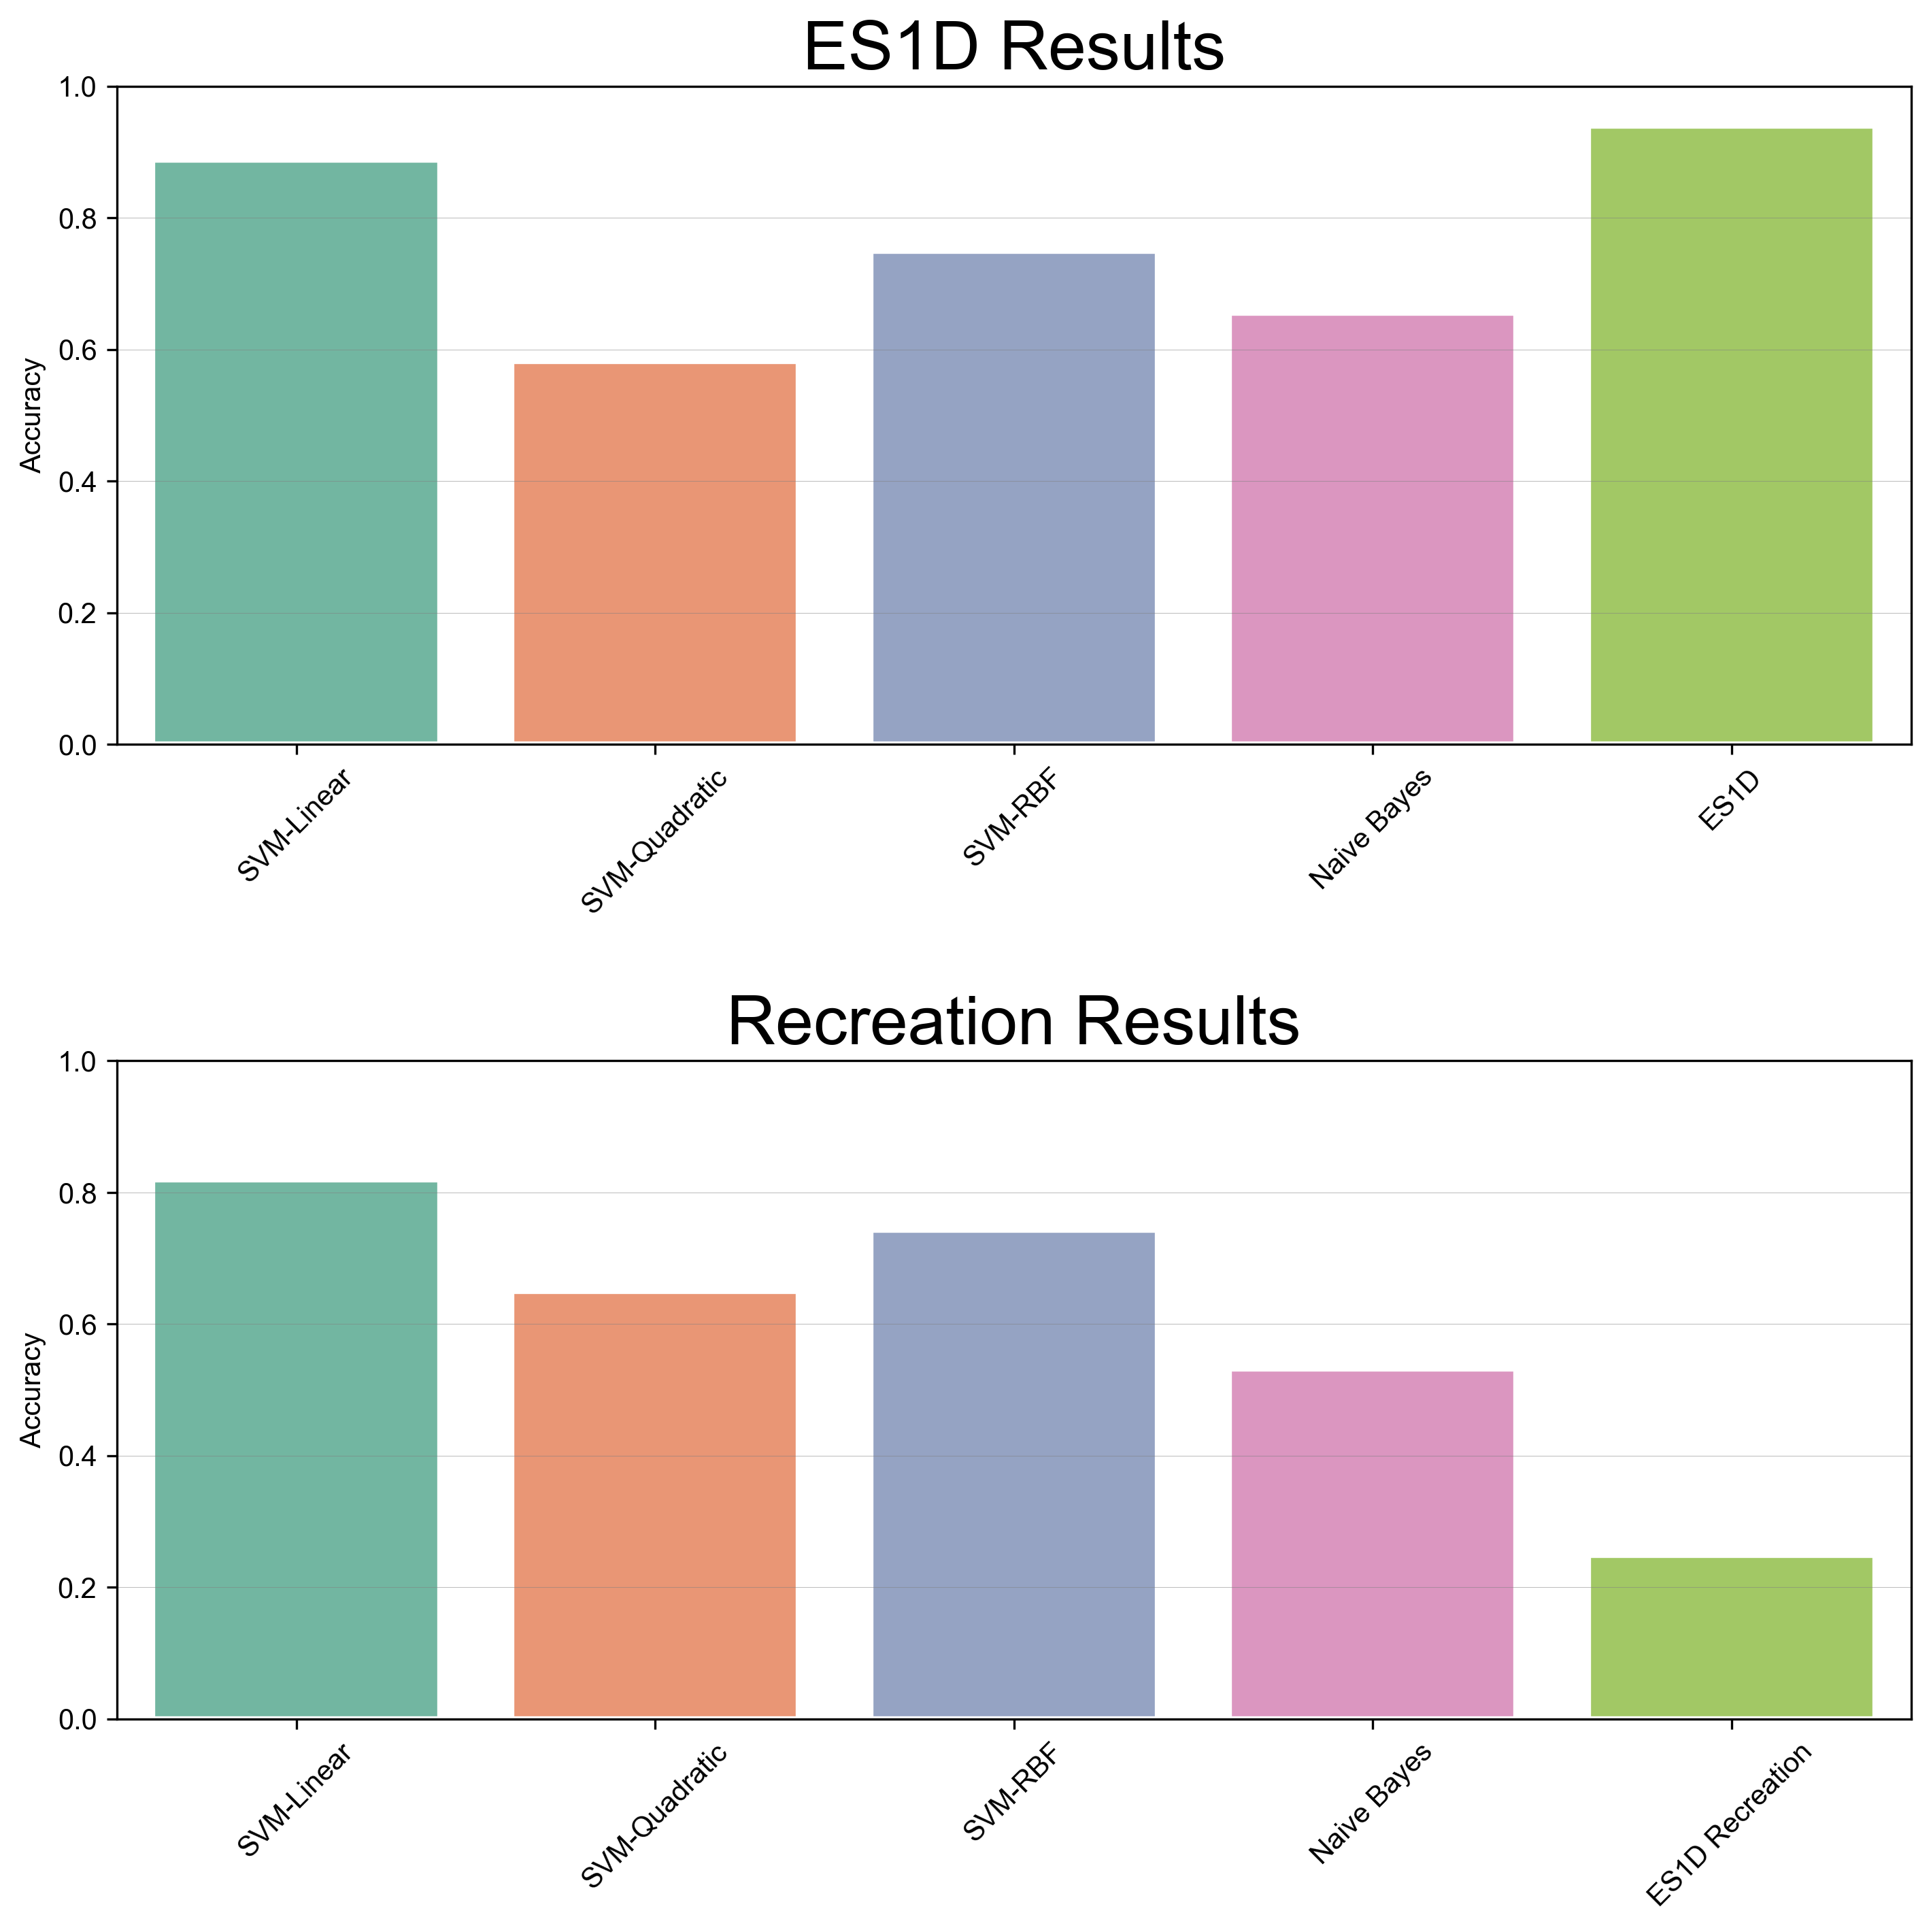
\includegraphics[width=0.5\textwidth]{results.png}
        \caption{\small{ES1D and recreation classification results}}
        \label{fig:results}
    \end{figure}
\end{center}
The first factor to consider comes from the differences in the dataset being used.
Since the DREAMER dataset was focused on recording ERPs, a larger percentage of the signals analyzed in ES1D may have been weighted in their favor.
As the studies above have shown, biometric information classification of ERP signal segments is much easier than classification of the entire EEG signal\cite{Review,Cerebre,TransformerNetworks,Brainprint,Imagined}.
This could be compounded by the fact that the two datasets had different sampling rates.
In this work, this was compensated by reevaluating the input size for the model architecture and creating scripts so that the data extraction process would fit.

It should also be noted that there are slight differences caused by missing information in the preprocessing and feature extraction phase.
Most notably, the lack information about artefact removal, as if ICA was used in the original work, this would strongly impact the PSD estimation, since Welch's method finds average values of the PSD over a window.
All other proportional window sizes and strides were kept the same, but the recreation did not use ICA at all. This could have diminished the accuracy of the recreation model.

The next point of consideration is the lack of computing time and resources available to the recreation.
Since the original ES1D model was able to train for 1,000,000 iterations, there is a strong possibility that this gave way to the model's success.
Additionally, since the ES1D model utilized holdout validation but had sourced the evaluation and training data from the same subjects, there is a chance that the model was overfitting to the data.
If that were the case, the recreation's lack in accuracy would make sense, as their model has not yet been shown to generalize.

Additionally, if more information about hyperparameter tuning had been provided in the original paper, there is a chance that the recreation could have been more successful.
While this is unlikely to have made a significant difference since most of the hyperparameters were set to default values, it is still a possibility.
\section{Conclusion}
In conclusion, the recreation attempt did not produce a classifer as successful as the original ES1D, but going through the full process did teach me many lessons about machine learning research.
I did not really know what values to look for when researching a study, so the intitial ES1D paper did not raise any red flags for me.
But I now know that I need to ensure that implementation details like the hyperparameters used are included in the paper.
This process also helped me to understand the difficulties that can be faced in something as simple as data pipelining.
From handling file inconsistencies, to acccounting for missing information, personally scripting solutions for this process was a great learning experience.
I plan to continue tuning this model in the hopes that it eventually classifies comparably to the original ES1D model.
I also plan to test the model on the DREAMER dataset to see if the results are any different, though I am still unlikely to run said experiment for 1,000,000 iterations.

This has been a wonderful learning experience, and I am incredibly grateful to have taken this class. 
The entire teaching team deserves a round of applause for their hard work and dedication to helping us learn.
I would also like to thank my classmates for their support and encouragement throughout the semester.